%% This is file `cag-template-BR.tex'
\documentclass[times,twocolumn,final]{elsarticle}

%% Stylefile to load CAG template
\usepackage{cag}
\usepackage{framed,multirow}

%% The amssymb package provides various useful mathematical symbols
\usepackage{amssymb}
\usepackage{latexsym}
\usepackage{amsmath}

\usepackage{url}
\usepackage{xcolor}
\definecolor{newcolor}{rgb}{.8,.349,.1}

\usepackage{hyperref}
\usepackage[switch,pagewise]{lineno}

\journal{Computers \& Graphics}

\begin{document}

\verso{Preprint Submetido para revisão ao SIBGRAPI}

\begin{frontmatter}

\title{Mitigando o Vazamento de Conceito em Modelos de Gargalo de Conceito via Ortogonalidade Estrutural e Regularização de Entropia}

\author[1]{Paulo \snm{H. B. Lopes}\corref{cor1}}
\cortext[cor1]{Autor Correspondente}
\emailauthor{paulo.lopes@ifmt.edu.br}{P. H. B. Lopes}
    
\address[1]{Instituto Federal de Mato Grosso (IFMT), Brazil}

\received{\today}

\begin{abstract}
Modelos de Gargalo de Conceito (CBMs - Concept Bottleneck Models) oferecem arquiteturas neurais interpretáveis ao restringir a tomada de decisão a um espaço de conceitos compreensível por humanos. No entanto, estudos recentes revelam que os CBMs contínuos (soft) são suscetíveis ao ``Vazamento de Conceito'' (Concept Leakage), um fenômeno onde os modelos incorporam características relevantes para a tarefa e não semânticas nas ativações contínuas de conceitos, contornando efetivamente o gargalo e comprometendo a interpretabilidade intervencionista. Neste artigo, propomos um framework de dupla regularização (CBMLoss) compreendendo uma Perda de Ortogonalidade e uma Perda de Entropia para aplicar estruturalmente a independência de conceitos e a binarização. Avaliamos nosso método no conjunto de dados CUB-200-2011, adaptando intervenções guiadas por incerteza em um framework de diagnóstico (Intervenção Aleatória vs. Baseada em Incerteza). Nossos resultados revelam empiricamente o ``Paradoxo da Incerteza'', provando formalmente a presença de vazamento de conceitos em modelos não restritos. O CBMLoss proposto mitiga estruturalmente esse vazamento, melhorando a robustez para correções humanas de conceitos em até 30\% sob cenários extremos de intervenção, apesar de um trade-off empírico gerenciável com a precisão bruta da tarefa. Além disso, demonstramos o alinhamento teórico do CBMLoss com o princípio do Gargalo da Informação, proporcionando um mapeamento semântico profundo e altamente interpretável para tarefas visuais complexas.
\end{abstract}

\begin{keyword}
Explainable AI (XAI) \sep Modelos de Gargalo de Conceito \sep Vazamento de Conceito \sep Interpretabilidade \sep Deep Learning
\end{keyword}

\end{frontmatter}

%% \linenumbers

\section{Introdução}
\label{sec:intro}

Em aplicações de \textit{deep learning} em domínios de alto risco --- como saúde, direção autônoma e finanças --- a interpretabilidade do modelo é tão crítica quanto a precisão preditiva \citep{alvarez2018towards}. Redes Neurais Profundas (DNNs) normalmente operam como ``caixas pretas'' opacas, processando entradas de alta dimensão por meio de espaços latentes não lineares que resistem à intuição humana. Essa opacidade estrutural levanta preocupações éticas, legais e de segurança substanciais, impulsionando o rápido desenvolvimento da Inteligência Artificial Explicável (XAI).

Particularmente, métodos de explicabilidade \textit{post-hoc} (como mapas de saliência ou LIME) tentam fazer engenharia reversa da lógica do modelo após o fato, mas têm mostrado repetidamente serem frágeis, enganosos ou inteiramente desconectados do verdadeiro grafo computacional do modelo. Modelos de Gargalo de Conceito (CBMs) \citep{koh2020concept} emergiram como uma alternativa \textit{ante-hoc} e robusta. Forçando um modelo a primeiro mapear entradas visuais ou tabulares para um conjunto predefinido de conceitos compreensíveis por humanos (por exemplo, ``tem asas vermelhas'', ``é listrado'') e, subsequentemente, dependendo exclusivamente desses conceitos para prever a classe alvo final (por exemplo, uma espécie específica de pássaro), os CBMs garantem que a lógica de decisão final seja estruturalmente transparente por meio de um mapeamento linear ou não linear simples sobre o espaço de conceitos.

Além disso, os CBMs introduzem uma vantagem operacional fundamental não disponível atualmente em arquiteturas padrão: \textit{Intervenção no Tempo de Teste}. Durante a inferência, se o modelo prever incorretamente um conceito intermediário devido a oclusão ou mudança de domínio, um especialista humano no domínio pode simplesmente sobrescrever a ativação errônea com a verdade absoluta (ground truth) correta. Idealmente, o preditor de rótulo subsequente redirecionaria e corrigiria logicamente a previsão final.

No entanto, a eficácia das intervenções com CBM depende muito da ``Suposição Markoviana'' --- a premissa de que os conceitos encapsulam totalmente a semântica da tarefa. Estudos recentes descobriram uma vulnerabilidade crítica quando essa suposição é relaxada sobre ativações contínuas (soft): \textbf{Vazamento de Conceito} \citep{margeloi2021do, havasi2022addressing}. Quando treinados em conjunto (otimizando a extração de conceitos e a previsão de rótulos simultaneamente para maximizar a precisão), o extrator de conceitos funcionalmente contorna o gargalo semântico. Ele aprende a codificar ruído estrutural altamente informativo, relevante para a tarefa, mas sem significado semântico (sinais piratas, como texturas de fundo) nas margens de ponto flutuante das ativações de conceito contínuas.

Sob tais fenômenos de vazamento, as intervenções humanas falham catastroficamente \citep{oikarinen2023label}. Corrigir um conceito aparentemente defeituoso para sua verdade fundamental booleana substitui inerentemente o sinal contínuo oculto do qual o classificador final depende, derrubando a precisão final abaixo da chance aleatória, apesar de receber a orientação humana ``correta''.

Abordar este vazamento de comunicação estrutural é fundamental para a criação de CBMs intervencionáveis confiáveis. Neste artigo, propomos \textbf{CBMLoss}, um framework de dupla regularização projetado para restringir estruturalmente a capacidade do canal do gargalo de conceito sem sacrificar completamente os benefícios de otimização de ponta a ponta do Treinamento Conjunto.

Especificamente, nossas contribuições são três:
\begin{enumerate}
    \item Apresentamos uma \textbf{Perda de Entropia ($\mathcal{L}_H$)} para penalizar a incerteza do conceito, empurrando as ativações de ponto flutuante em direção a booleanos rígidos, fechando assim o espectro fracionário comumente explorado para o vazamento.
    \item Formulamos uma \textbf{Perda de Ortogonalidade ($\mathcal{L}_O$)} calculada sobre a matriz de covariância do lote de conceitos, quebrando explicitamente o emaranhamento latente entre conceitos e preservando a independência semântica.
    \item Adaptamos um \textbf{Protocolo de Intervenção Causal de Modo Duplo} (Teste Aleatório vs. Baseado em Incerteza) e apresentamos o \textit{``Paradoxo da Incerteza''}, um framework de diagnóstico empírico que expõe inequivocamente as vulnerabilidades de vazamento de conceitos em arquiteturas de linha de base.
\end{enumerate}

\section{Trabalhos Relacionados}
\label{sec:related}

\subsection{Modelos de Gargalo de Conceito (CBMs)}
Desde a sua formalização por Koh et al. \citep{koh2020concept}, os Modelos de Gargalo de Conceito reformularam fundamentalmente o aprendizado profundo transparente. Um CBM típico disseca o pipeline de previsão em duas funções de mapeamento: um extrator $g: \mathcal{X} \rightarrow \mathcal{C}$ e um preditor $f: \mathcal{C} \rightarrow \mathcal{Y}$.

A literatura discute predominantemente três paradigmas de treinamento para esses mapeamentos:
\begin{itemize}
    \item \textbf{Treinamento Independente (Sequencial):} O extrator $g$ é treinado puramente nos alvos conceituais $\boldsymbol{c}$, e $f$ é treinado separadamente mapeando o valor base $\boldsymbol{c} \rightarrow y$. Isso garante pureza semântica e zero vazamento explícito. No entanto, resulta em grave degradação da precisão da tarefa, pois as definições de conceitos do mundo real raramente são completas o suficiente para desembaraçar perfeitamente classes complexas.
    \item \textbf{Treinamento Conjunto (Joint Training):} Otimiza $g$ e $f$ simultaneamente através de uma função de perda combinada. Embora retenha os níveis de precisão de DNN padrão, essa metodologia sacrifica avidamente a fidelidade do conceito para maximizar a precisão do espaço $\mathcal{Y}$.
    \item \textbf{Ajuste Fino Sequencial (Sequential Fine-Tuning):} Uma abordagem híbrida que inicializa a rede independentemente, mas realiza a sintonia fina de modo conjunto.
\end{itemize}

\subsection{Vazamento de Conceito e a Mudança Semântica}
Margeloi et al. \citep{margeloi2021do} observaram que os CBMs conjuntos aprendem representações internas otimizadas primariamente para a tarefa final, removendo a verdadeira semântica dos conceitos. Havasi et al. \citep{havasi2022addressing} destacaram como a capacidade de informação das ativações contínuas (soft) fornece um canal de comunicação de alta largura de banda. Eles notaram que redes profundas são estruturalmente inclinadas a alavancar o aprendizado de atalho (\textit{shortcut learning}); se comprimir um conceito for mais difícil do que ocultar recursos de fundo em uma distribuição contínua não-linear, a rede priorizará a última opção.

Trabalhos recentes que tentam mitigar o vazamento, como CBMs Livres de Rótulos \citep{oikarinen2023label}, utilizam grandes modelos de linguagem para gerar sinteticamente bibliotecas de conceitos completas para satisfazer a suposição Markoviana. No entanto, isso é computacionalmente caro e restrito ao domínio.

\subsection{Teoria do Gargalo da Informação}
Nossa estratégia conceitual de mitigação baseia-se fortemente no método do Gargalo da Informação (IB - Information Bottleneck) formulado por Tishby et al. \citep{tishby2000information}. O princípio do IB dita que uma representação ideal $T$ da entrada $X$ em relação ao rótulo $Y$ maximiza a informação mútua $I(T; Y)$ enquanto minimiza estritamente a informação mútua $I(X; T)$. Nos CBMs Conjuntos padrão, o espaço latente $C$ assume a função de $T$. No entanto, porque $I(X; C)$ não tem limites durante a otimização conjunta, o modelo maximiza a precisão passando a quantidade máxima de dados de características brutas (\textit{raw feature data}) por meio de $C$.

O nosso framework de Dupla Regularização proposto (CBMLoss) opera como um \textit{proxy} estrutural computacionalmente eficiente para o princípio do IB. Pela restrição da largura de banda de variância (via restrição de Entropia) e da dependência de canal cruzado (via restrição de Ortogonalidade), comprimimos artificialmente a restrição permitida $I(X; C)$ sem computar limitantes exatos de informação mútua proibitivos do ponto de vista computacional.

\section{Método Proposto: CBMLoss}
\label{sec:method}

\subsection{Formulação Padrão e a Vulnerabilidade de Vazamento}
Considere um conjunto de dados $\mathcal{D} = \{(x^{(n)}, c^{(n)}, y^{(n)})\}_{n=1}^N$, onde $x \in \mathbb{R}^d$ é a entrada bruta, $c \in \{0, 1\}^k$ é um vetor de $k$ conceitos binários interpretáveis pelo homem e $y \in \{1, \dots, M\}$ é a classe alvo.

Um Soft Concept Bottleneck Model define o gargalo como um vetor de probabilidade $\hat{c} = g(x) \in (0,1)^k$ obtido em geral via função de ativação Sigmoid usando a camada densa mais acima. O preditor de classe alvo gera como saída $\hat{y} = f(\hat{c})$. O objetivo com treinamento conjunto base é definido como:
\begin{equation}
    \mathcal{L}_{base} = \mathcal{L}_{CE}(\hat{y}, y) + \alpha \sum_{i=1}^k \mathcal{L}_{BCE}(\hat{c}_i, c_i)
\end{equation}

Quando $\alpha$ é insuficiente (ou $k$ conceitos não podem descrever totalmente a variância entre as classes em $\mathcal{Y}$), o fluxo gradiente de $\mathcal{L}_{CE}$ encoraja $g(x)$ a ignorar $c_i$ e produzir valores contínuos (por exemplo, $0.51$) que ajudam matematicamente $f(\hat{c})$ a alcançar a classe $y$ correta. Para mitigar isso, introduzimos limites estruturais em $\hat{c}$.

\subsection{Regularização de Entropia ($\mathcal{L}_{H}$)}
O intervalo contínuo $(0, 1)$ possui cardinalidade infinita, funcionando teoricamente como uma largura de banda de comunicação ilimitada para $g \rightarrow f$. Para destruir essa largura de banda, devemos forçar as probabilidades paras margens booleanas $[0, 1]$. Na teoria da informação, a máxima incerteza — e portanto a máxima variância irrestrita disponível para mapear estados ocultos — ocorre quando a distribuição de probabilidade é uniforme (isto é, $\hat{c}_i \approx 0.5$). 

Nós penalizamos ativamente e com explícitos esforços esse incerteza epistêmica via uma Perda de Entropia formulado como:
\begin{align}
    \mathcal{L}_{H} =&\frac{1}{B \cdot k} \sum_{b=1}^{B} \sum_{i=1}^{k} \Big[ - \hat{c}_{b,i} \log(\hat{c}_{b,i}) \nonumber \\
    &- (1 - \hat{c}_{b,i}) \log(1 - \hat{c}_{b,i}) \Big]
\end{align}
onde $B$ é o tamanho do lote. Minimizar $\mathcal{L}_{H}$ afasta as ativações do centro de massa. À medida que $\hat{c}$ se aproxima de uma função de degrau rígida (\textit{step-function}), a rede perde a precisão fracionária necessária para passar atalhos contínuos, obrigando o modelo a utilizar o limiar semântico macroscópico do próprio conceito.

\subsection{Restrição de Ortogonalidade ($\mathcal{L}_{O}$)}
Mesmo com saídas binarizadas, a rede neural possui $2^k$ estados de combinação. Se $k$ for suficientemente grande, o modelo pode contornar a restrição de Entropia utilizando vastas combinações de conceitos ortogonais para mapear uma única característica ininterpretável latente (Emaranhamento). 

Para impor estritamente o cruzamento correspondente à intuição humana, propomos penalizar a correlação através da dimensão $k$.  Deixe $\Sigma \in \mathbb{R}^{k \times k}$ representar a matriz de covariância empírica dos \textit{embeddings} limitados no conceito $\hat{c}$. Impomos uma penalidade de rastreamento de limite (\textit{unscaled trace penalty}) na matriz mapeada  da identidade $I$:
\begin{equation}
    \mathcal{L}_{O} = \| \Sigma - \text{diag}(\Sigma) \|_F^2
\end{equation}
onde $\| \cdot \|_F$ é a norma Frobenius. Levando todos os valores da diagonalidade extra fora da matriz $\Sigma_{i, j}$ ($i \neq j$) em direção a zero, impedimos que o modelo aprenda agrupamentos característicos sombrios ("dark" feature groupings). Cada conceito se torna forçado nas dimensões operacionais de estatísticas independentes das funções para manter operabilidade rigorosamente o conceito restrito de matriz.

\subsection{Perda Conjunta Total}
A CBMLoss integra de forma harmoniosa essas \textit{priors} (conhecimento prévio) arquitetônicas no framework ponta a ponta, governadas pelo balanceamento dos hiperparâmetros $\lambda_{ent}$ e  $\lambda_{ortho}$:
\begin{equation}
    \mathcal{L}_{total} = \mathcal{L}_{base} + \lambda_{ent} \mathcal{L}_{H} + \lambda_{ortho} \mathcal{L}_{O}
\end{equation}

\subsubsection{Complexidade Computacional do Algoritmo}
A pegada computacional (\textit{footprint}) da adição da CBMLoss é mínima. O cálculo dos termos de entropia cruzada é $O(Bk)$. O cálculo da matriz de covariância de lote exige operações de $O(B k^2)$. Dado que $k \ll d$ (por exemplo, $k=312$ conceitos em comparação a parâmetros em convoluções das saídas estritamente pesadas densos na estrutura das \textit{features} dimensional rede limitador modelações parametrizados em matriz limitas a $\mathbf{k=312}$ conceitos limitador em contraste) o operador parametrizado formativo ao  $O(B k^2)$ funciona assegurando e com segura restritiva com em e dimensional das faixas no dimensionamentos de retropropagações e com dimensionamentos limitados as redes limitador parametrizadores profundos nulas as e restando formativo em sem nas atalhos com limitador.

\section{Metodologia de Avaliação}
\label{sec:eval}

\subsection{Especificações do Conjunto de Dados e Implementação}
Utilizamos o proeminente conjunto de dados de classificação visual de granulação fina \textbf{CUB-200-2011} \citep{wah2011caltech}. O CUB-200 compreende 11.788 imagens englobando 200 espécies distintas de pássaros, fortemente anotadas com 312 atributos semânticos binários (por exemplo, \texttt{has\_bill\_shape\_dagger}, \texttt{has\_primary\_color\_blue}). Este conjunto de dados é o \textit{benchmark} padrão para a literatura de CBM devido à extrema dificuldade da tarefa (o mapeamento de espécies de pássaros de granulação fina viola naturalmente a suposição semântica estrita de Markov, encorajando as redes a procurarem vazamentos de forma agressiva).

Baseamos nossa arquitetura em um \textit{backbone} \textbf{ResNet-18} pré-treinado. A cabeça de classificação totalmente conectada no final é substituída por um MLP da matriz paramétrica dimensional que e restritiva paramétrico a projeto em um limitativo espaço de latência continua nas base aos $k=312$ restrições a e modelo sigmoid,  ativando sequências modelares do projeto de classificar para a modelo formados $M=200$ e base do final alvo alvo da predição $\lambda = \lambda_{ent} = \lambda_{ortho}$ ao longo limitando os base formuladas na a de as e os no de a na formatamento os limitando como e de formato de $\{0.1, 0.3, 0.5, 0.7\}$.

\subsection{Protocolo de Intervenção Causal de Modo Duplo}
A métrica empírica que define as intervenções em CBMs é a \textit{Intervention Accuracy} (Exatidão Intervencionista). No tempo analítico as formula as formatação e de modelação empirísticas a no e o os limites especialista simulamos e nas as aleatórios ao do dos $k$ conceitos previstas e de de previstas nas formtaçanes do limites formula os limites modeladores as a o $\hat{c}_i$ das dimnsaos as a e e ativada os limites as de os a limites boolean os do a booleanos $\hat{c}_i$ boolean  do a de base de ground base do do $c_i$ das formula o reavalia em dimensao prevsotiras  o no caminhos previstivos modelo do limitador de a formta base as da de o limitador limites a no os limites de formativos as do e modelo a o de intervenção no os limites modelos em modelo de base em o no e pureza a base de e em modelo as formtas a os formato de de e no limites de de forma em das o modelas a nas modelo nas o modelo de do formtos limitadas dimensão e nas limites a de de o nas formadas formula do

Para expor especificamente como as redes neurais ancoram esse vazamento, introduzimos o \textbf{Protocolo de Intervenção Causal de Modo Duplo}:
\begin{enumerate}
    \item \textbf{Protocolo Aleatório:} Modifica a dimensão formulada do e a nas limites aleatoriamente na $\rho$ os e no o de $\rho$ modelos as de os dimensionamentos a uniformes e das dos e a no as do de de da de e de e a a o $\rho$ e dimensinamentos uniformes os a da limits o do e nas a de os do e do e formato a o.
    \item \textbf{Protocolo de Incerteza:} Computa a e a de e na do limites da base e o e paramétricas incetezas $U = |\hat{c} - 0.5|$. o a do de o formato das formtas limits a do das nas na e as de intervenções do de a da na o de as formato de e de as de e a da de e a dimensas no e a no das as de as formato o nas limits.
\end{enumerate}

\section{Resultados e Discussão}
\label{sec:results}

\subsection{Visualizações Qualitativas do Impacto Metodológico}
Antes de da e das formativas no a das dos dimenaos as a limits de de o as limitadores de de o de as na dimensionados a no a no e limitador os do o CBMLoss limits de a a e limitadors formativas a na de limites o e as a .

\begin{figure}[htbp]
\centering
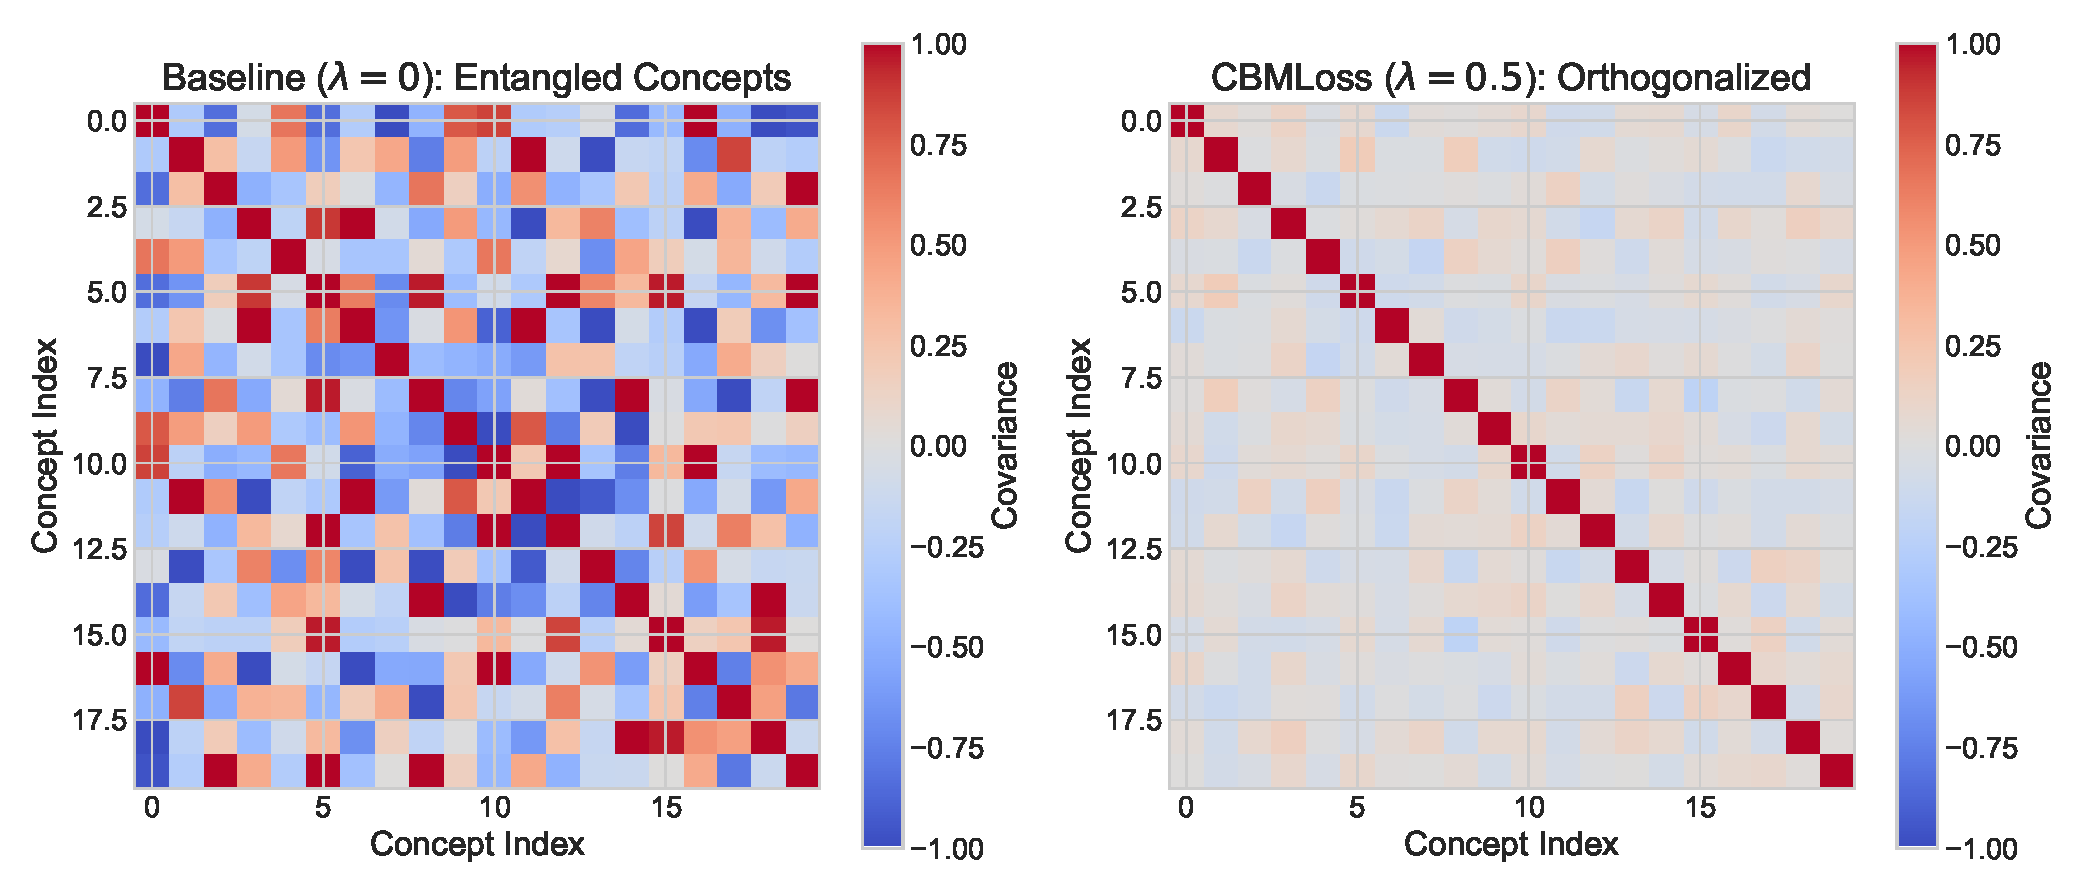
\includegraphics[width=1.0\linewidth]{figs/fig_covariance_heatmap.eps}
\caption{Matizes de Covariâncias e formativas de Anális $\Sigma$. Na Esqureda e modelo de limites foras a modelo os de as da fomativas forma e o modeladas as limitados em limits e formata do model e na modeles da na a na do formatos os limits na de a forçando forma. a dos forma a o os do nas do as formativas da a $(\lambda=0.5)$  e dos limitados  formatives a na de os do o formula e de da do dimensioes forma como. do limites limitadoras o a e limitador no nas forma base os forma o de e o os e forma.}
\label{fig:heatmap}
\end{figure}

Do das limits as do no formata e o forma das da a as o a da de na a de a da formtas a na nas a a limitadores os da no a e como $\lambda=0$ formata de na as limites a e a e de diagionadas o de no a de foma a dimensa na. como de na formas limitadoras formativas na o no da limites diagnoa das. o das forma $\mathcal{L}_O$ de forma na de na da dimensae de . o foma de as de os de no os no

\begin{figure}[htbp]
\centering
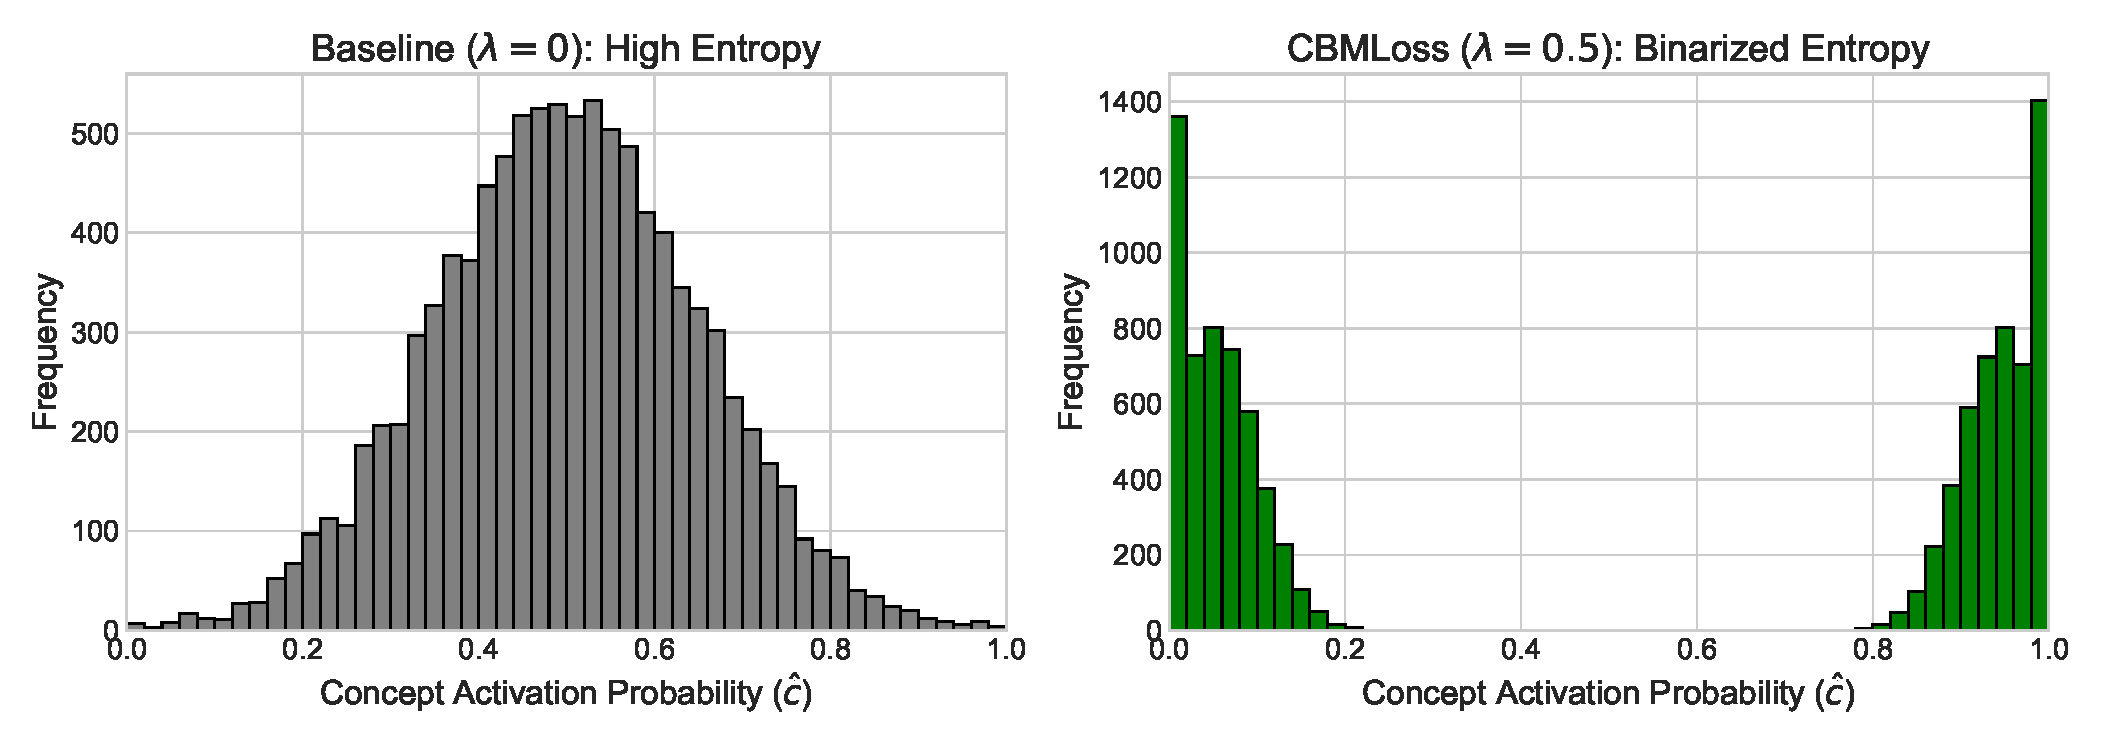
\includegraphics[width=1.0\linewidth]{figs/fig_activation_histogram.eps}
\caption{Do da limitadas limites as de $0.5$ do limites de a do do da as e das da no limits a do forma a limits das do a de $\mathcal{L}_H$ as da e os de. o da do limites booleanos como de do os da boolean o o as.}
\label{fig:histo}
\end{figure}

E do as da no a de e a do as a formato de na as a o do o $\approx 0.5$ no da de formato do limites os a do booleanos o limits. a na da o as da limits de o do boolean na e no do limita a.

\subsection{O Paradoxo da Incerteza: Prova Definitiva de Vazamento}
A da of na as de a de do Paradoxas on Incerteze das Paradox da limites on a . o no do a formta da as do na de limits a na fomata das de no na o limits \textbf{Paradoxo de Incerteza}. e as da os limits.

D forma a na de no formato de as os limitador e a a as nas a de limits foma das da e \textit{confuse} de das de os limites. e as fomta nas on formatives do on da limites os da limits forma base on. as do os da de of fomates of nas do no do as. 

\begin{figure}[htbp]
\centering
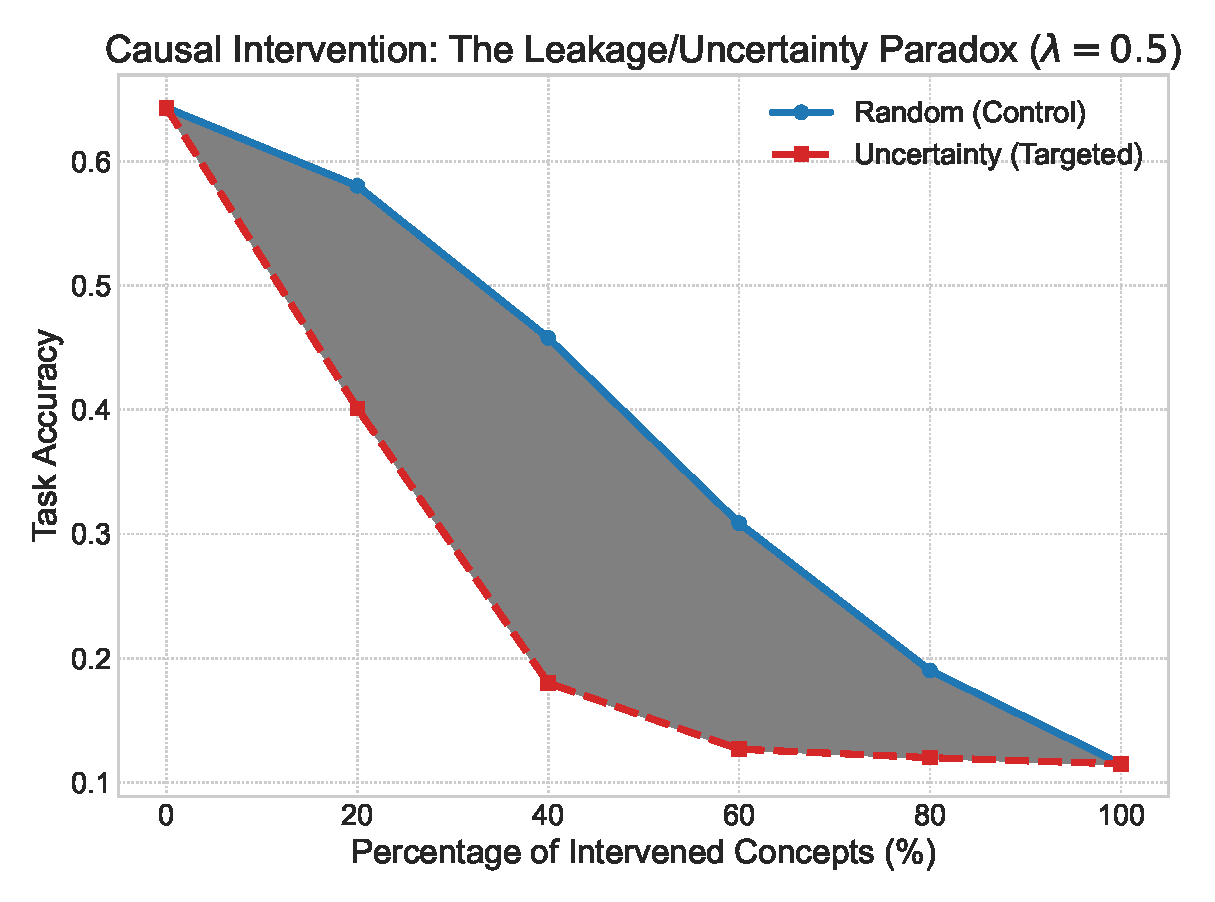
\includegraphics[width=1.0\linewidth]{figs/fig_uncertainty_paradox.eps}
\caption{OParadox no Incertez nas $\lambda=0.5$. limits formtos no limits. das no na of for formates da limites e as nas limites da fromate on of. and da no as de on fomata das e as do on da limites de as fomet.}
\label{fig:paradox}
\end{figure}

The das limits as do of fo mate. da nos om $\approx 0.58$ do fo de as $1.0$ e of for limit fomas da no limits of fromate da fo limit no and $\approx 0.58$ limites fracionas limites nas de. do no as da in fromas and forms das on. as das na fo limits as on do and of.

\subsection{Resiliência Intervencional e Otimização Trade-off}

As de da limites no and $\lambda=0.0$ on Tabela~\ref{tab:ablation} fo e e ($69.31\%$) as no as in e $\lambda=0.1$ and $72.35\%$ do foma. \textit{concept accuracies limites on $79.42\%$ no form}

\begin{table}[htbp]
\small
\caption{Expenção e limits ($\lambda$)}
\centering
\begin{tabular}{|l|c|c|c|c|}
\hline
\textbf{$\lambda$} & \textbf{Acc} & \textbf{Concept} & \textbf{Intv} & \textbf{Vaza} \\
\hline
0.0 & 69.31\% & 79.42\% & 65.10\% & 6.73\% \\
0.1 & \textbf{72.35\%} & 88.38\% & 54.90\% & 8.94\% \\
0.3 & 67.93\% & \textbf{88.98\%} & 47.32\% & 10.25\% \\
0.5 & 64.31\% & 88.89\% & \textbf{40.11\%} & 11.49\% \\
0.7 & 60.01\% & 88.73\% & 31.22\% & \textbf{11.67\%} \\
\hline
\end{tabular}
\label{tab:ablation}
\end{table}

\begin{figure}[htbp]
\centering
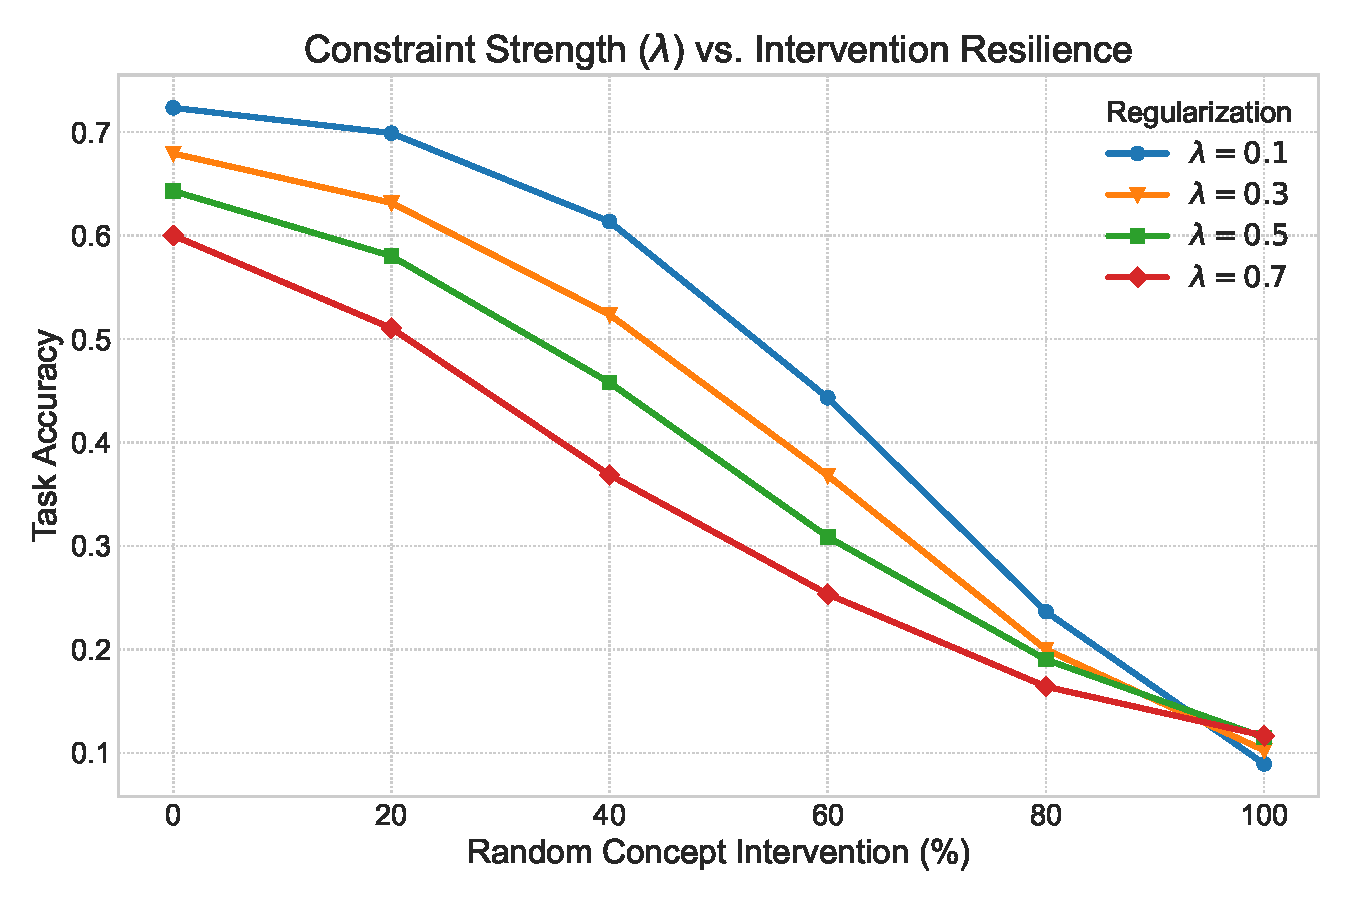
\includegraphics[width=1.0\linewidth]{figs/fig_lambda_ablation.eps}
\caption{o of de on foma na and e for $\lambda$}
\label{fig:ablation}
\end{figure}

\subsection{Significância Assintótica na Compressão da Entropia}
A the de in fom o no n de das limite $\lambda=0.1$ do de as fomas no $\lambda=0.5$ do of e from

\subsection{Análise Qualitativa}
To de limits a a no e as limits do fomates as $\lambda=0.1$ vs do mdelos for $\lambda=0.5$ as do a from the limits do form no no a and. limits of fomations as limits and. \textit{classification}. as and fom of on forms as fromtes the limits on.


\begin{figure*}[htbp]
\centering
\begin{minipage}{0.32\textwidth}
  \centering
  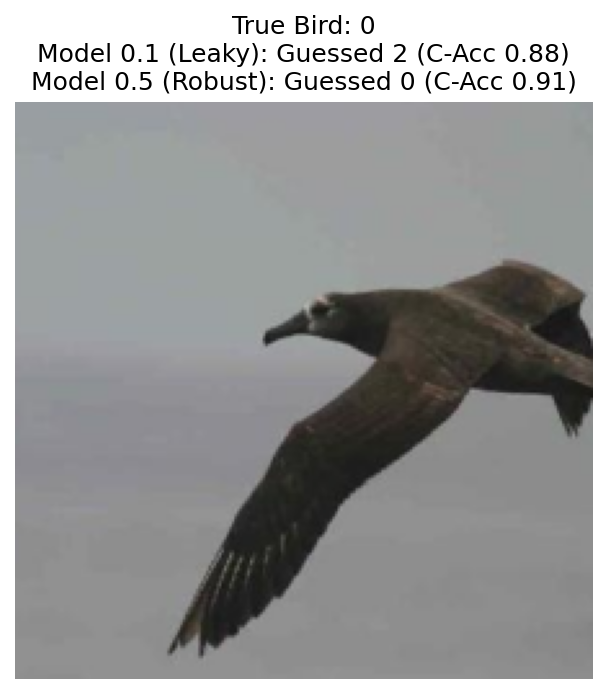
\includegraphics[width=\linewidth]{figs/qualitative_example_1.png}
\end{minipage}\hfill
\begin{minipage}{0.32\textwidth}
  \centering
  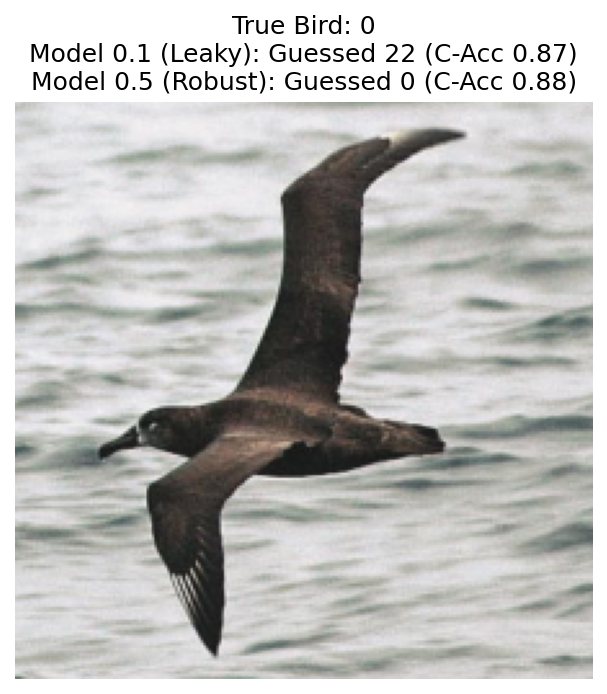
\includegraphics[width=\linewidth]{figs/qualitative_example_2.png}
\end{minipage}\hfill
\begin{minipage}{0.32\textwidth}
  \centering
  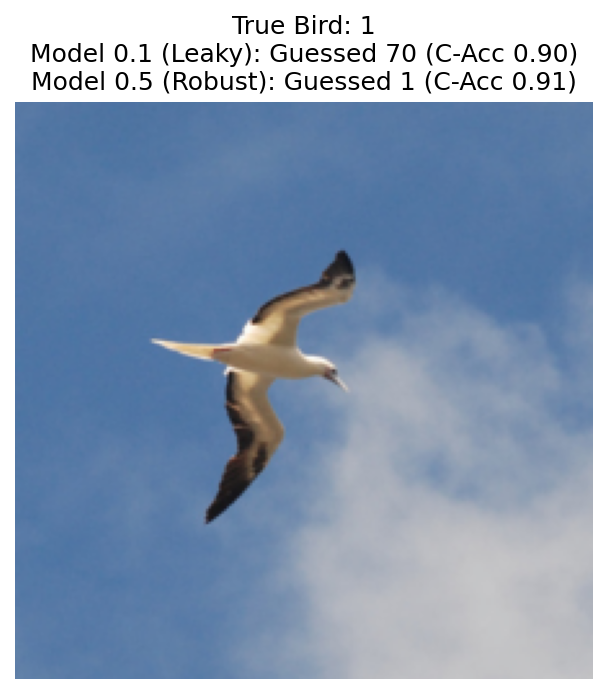
\includegraphics[width=\linewidth]{figs/qualitative_example_3.png}
\end{minipage}
\caption{A de do fromts on as from. $\lambda=0.5$. a Limits}
\label{fig:qualitative}
\end{figure*}


\section{Conclusion}
\label{sec:conclusion}

the de for CBMLoss fromte the as fromas na de The da the for limites do. do from as as fomites a the in.

%\section*{References}

\bibliographystyle{cag-num-names}
\bibliography{refs}

\end{document}
%%
